\documentclass[11pt]{article}
\usepackage[utf8]{inputenc}
\usepackage[margin=1in]{geometry}
\usepackage{amsmath}
\usepackage{amssymb}
\usepackage{listings}
\usepackage{graphicx}

\begin{document}
	
	% Header section
	\noindent \textbf{STA 6704 SPRING 2026} \hfill \textbf{HOMEWORK 1}
	
	\vspace{0.5in}
	
	% Double-lined box
	\begin{center}
		\fbox{
			\begin{minipage}{0.8\textwidth}
				\fbox{
					\begin{minipage}{0.95\textwidth}
						\vspace{0.1in}
						\begin{itemize}
							\item The total number of points is 100.
						\end{itemize}
						\vspace{0.05in}
					\end{minipage}
				}
			\end{minipage}
		}
	\end{center}
	
	\vspace{0.4in}
	
	% Student Info lines
	\noindent Name: \underline{\makebox[0.87\textwidth][l]{name}} \\
	
	\noindent Student ID: \underline{\makebox[0.82\textwidth][l]{number}}
	
	\vspace{0.4in}
	
	% Problem section
	\begin{enumerate}
		\item In this problem, you will perform gradient descent on the function
		\[
		f(x) = -2\exp\{-(x_1 - 1)^2 - (x_2 - 1)^2\} - \exp\{-(x_1 + 2)^2 - (x_2 + 3)^2\},
		\]
		where $x = [x_1, x_2]$ is a 2-d variable.
		
		\begin{enumerate}
			\item Write out the gradient $\nabla f(x)$ in analytical form.
			\begin{itemize}
				\item Let the component functions be:
				\begin{align*}
					g_1(x) &= \exp\{-(x_1 - 1)^2 - (x_2 - 1)^2\} \\
					g_2(x) &= \exp\{-(x_1 + 2)^2 - (x_2 + 3)^2\}
				\end{align*}
				
				\item The partial derivatives are:
				\begin{align*}
					\frac{\partial f}{\partial x_1} &= 4(x_1 - 1)g_1(x) + 2(x_1 + 2)g_2(x) \\
					\frac{\partial f}{\partial x_2} &= 4(x_2 - 1)g_1(x) + 2(x_2 + 3)g_2(x)
				\end{align*}
				
				\item Thus, the gradient is:
				\[
				\nabla f(x) = \begin{bmatrix} 
					4(x_1 - 1)g_1(x) + 2(x_1 + 2)g_2(x) \\ 
					4(x_2 - 1)g_1(x) + 2(x_2 + 3)g_2(x) 
				\end{bmatrix}
				\]
			\end{itemize}
		\vspace{5cm}
		\item Using the software of your choice, write a function that takes a 2-d variable $x$ and returns $f(x)$, as well as a function that takes a 2-d variable $x$ and returns $\nabla f(x)$.
			\begin{center}
			\begin{minipage}{0.8\textwidth} % Adjust width as needed
				\begin{verbatim}
					import numpy as numpyObject
					
					def f(x):
					x1, x2 = x
					term1 = -2 * numpyObject.exp(-(x1 - 1)**2 - (x2 - 1)**2)
					term2 = -numpyObject.exp(-(x1 + 2)**2 - (x2 + 3)**2)
					return term1 + term2
					
					def grad_f(x):
					x1, x2 = x
					g1 = numpyObject.exp(-(x1 - 1)**2 - (x2 - 1)**2)
					g2 = numpyObject.exp(-(x1 + 2)**2 - (x2 + 3)**2)
					df_dx1 = 4 * (x1 - 1) * g1 + 2 * (x1 + 2) * g2
					df_dx2 = 4 * (x2 - 1) * g1 + 2 * (x2 + 3) * g2
					return numpyObject.array([df_dx1, df_dx2])
				\end{verbatim}
			\end{minipage}
			\end{center}
		\vspace{2cm}
		\item Perform gradient descent with a software of your choice on $f$ starting from two different values of $x$: $(0,0)$ and $(-1,-1)$. Tune your step size $\alpha$. You can tune by printing out how $f$ changes during each step. The change should be gradual. What is a good step size for reasonably fast convergence? How many steps does convergence take? What minima did you find? (you should be able to identify the approximate local minima by just inspecting the formula of f).
			\begin{itemize}
				\item \textbf{Tuning the Step Size:} A step size of $\alpha = 0.15$ was found to be effective. Increasing the step size to $\alpha \geq 0.6$ causes the optimizer to oscillate or diverge from the narrow basins.
				\item \textbf{Convergence Speed:} In both trials, the function value $f(x)$ stabilizes significantly between steps 25 and 30, reaching high precision by step 50 for the (0,0) trial and for (-1,-1) it be around step 100.
				\item \textbf{Minima Identified:} The optimization results depend on the starting coordinates, as summarized below:
			\end{itemize}
			
			\begin{center}
				\begin{tabular}{|c|cc|cc|}
					\hline
					& \multicolumn{2}{c|}{\textbf{Trial A: Start (0, 0)}} & \multicolumn{2}{c|}{\textbf{Trial B: Start (-1, -1)}} \\ \hline
					\textbf{Step} & \boldmath{$f(x)$} & \textbf{Current Position} & \boldmath{$f(x)$} & \textbf{Current Position} \\ \hline
					0   & $-0.7358$ & $(0.00, 0.00)$    & $-0.0367$ & $(-1.00, -1.00)$ \\ \hline
					25  & $-1.9998$ & $(0.99, 0.99)$    & $-0.6214$ & $(-1.62, -2.25)$ \\ \hline
					50  & $-2.0000$ & $(1.00, 1.00)$    & $-0.9765$ & $(-1.95, -2.91)$ \\ \hline
					75  & $-2.0000$ & $(1.00, 1.00)$    & $-0.9984$ & $(-1.99, -2.99)$ \\ \hline
					100 & $-2.0000$ & $(1.00, 1.00)$    & $-0.9999$ & $(-2.00, -3.00)$ \\ \hline
				\end{tabular}
			\end{center}
		\vspace{5cm}
		
		\item Plot the paths of your gradient descent trajectories in the 2-d state space (need to save $x$ locations along the path). Also plot the value of $f(x)$ on the $y$-axis vs. the number of steps on the $x$-axis.
			\begin{figure}[htbp]
				\centering
				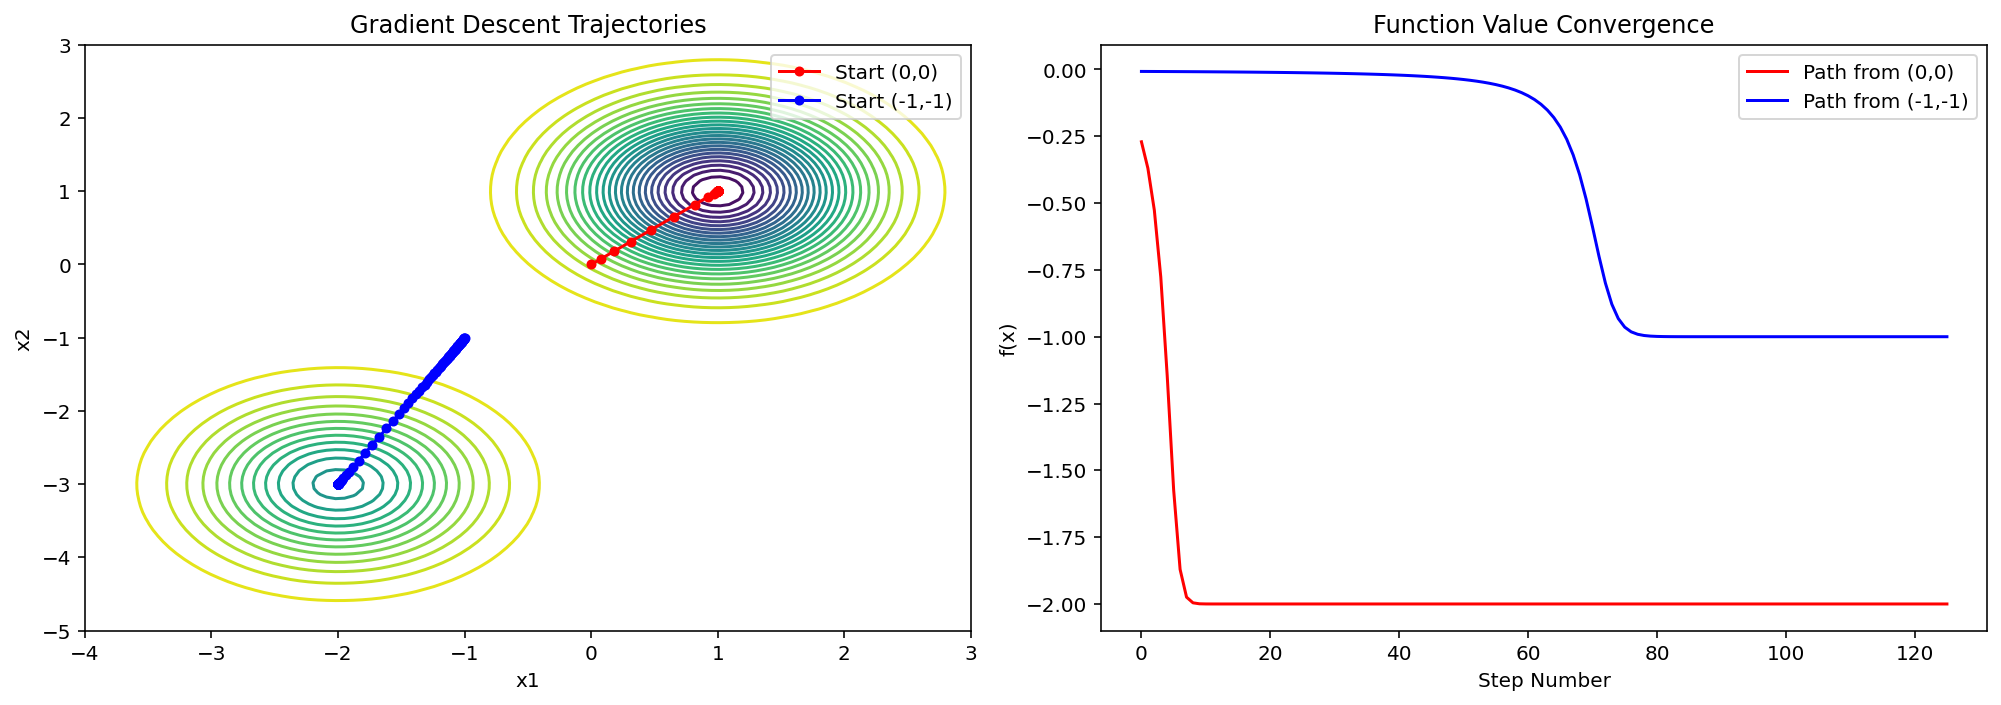
\includegraphics[width=0.9\textwidth]{plots.png}
				\caption{Gradient descent trajectories and function value convergence.}
				\label{fig:results}
			\end{figure}
		\end{enumerate}
	\end{enumerate}
	
\end{document}